\documentclass[tikz]{standalone}

\definecolor{n0}{HTML}{785EF0}
\definecolor{End}{HTML}{DC267F}
\definecolor{Reversal}{HTML}{FFB000}
\definecolor{NewHex}{HTML}{648FFF}
\definecolor{Corner}{HTML}{FE6100}

\begin{document}
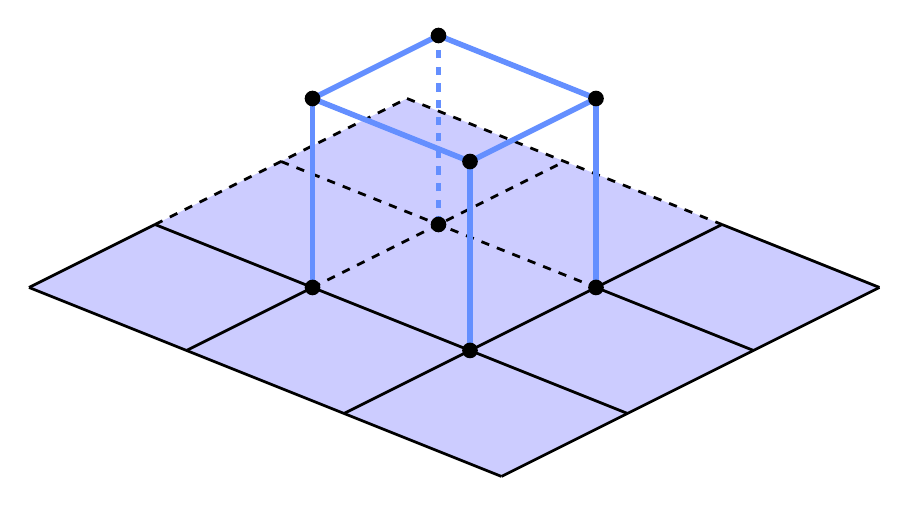
\begin{tikzpicture}[scale=4, x={(0.5cm,-0.2cm)}, y={(0.4cm,0.2cm)}, z={(0.0cm,0.6cm)}]

  %%%%%%%%%% Points pour travailler %%%%%%%%%%
 \coordinate (1) at (0,0,0) ;
 \coordinate (2) at (1,0,0) ;
 \coordinate (3) at (2,0,0) ;
 \coordinate (4) at (3,0,0) ;
 \coordinate (5) at (0,1,0) ;
 \coordinate (6) at (1,1,0) ;
 \coordinate (7) at (2,1,0) ;
 \coordinate (8) at (3,1,0) ;
 \coordinate (9) at (0,2,0) ;
 \coordinate (10) at (1,2,0) ;
 \coordinate (11) at (2,2,0) ;
 \coordinate (12) at (3,2,0) ;
 \coordinate (13) at (0,3,0) ;
 \coordinate (14) at (1,3,0) ;
 \coordinate (15) at (2,3,0) ;
 \coordinate (16) at (3,3,0) ;
 \coordinate (17) at (1,1,1) ;
 \coordinate (18) at (2,1,1) ;
 \coordinate (19) at (1,2,1) ;
 \coordinate (20) at (2,2,1) ;

 \fill [color=blue!20!white] (1) -- (4) -- (16) -- (13) -- cycle ;
 
 % Layer 1
 \draw [line width=1] (1) -- (4) ;
 \draw [line width=1] (5) -- (8) ;
 \draw [line width=1] (11) -- (12) ;
 \draw [line width=1] (15) -- (16) ;
 
 \draw [line width=1] (1) -- (5) ;
 \draw [line width=1] (2) -- (6) ;
 \draw [line width=1] (3) -- (15) ;
 \draw [line width=1] (4) -- (16) ;

 \draw [dashed, line width=1] (6) -- (14) ;
 \draw [dashed, line width=1] (13) -- (15) ;

 \draw [dashed, line width=1] (5) -- (13) ;
 \draw [dashed, line width=1] (9) -- (11) ;
 
 %%%%%%%%%%% The HEXA created %%%%%%%%%%%
 \draw [line width=2, color=NewHex] (17) -- (18) -- (20) -- (19) -- (17) ;
 \draw [line width=2, color=NewHex] (6) -- (17) ;
 \draw [line width=2, color=NewHex] (7) -- (18) ;
 \draw [dashed, line width=2, color=NewHex] (10) -- (19) ;
 \draw [line width=2, color=NewHex] (11) -- (20) ;

  %%%%%%%%%%% HEXA NODES %%%%%%%%%%%
 \draw (6) node[circle, fill=black, inner sep = 2 pt] {};
 \draw (7) node[circle, fill=black, inner sep = 2 pt] {};
 \draw (10) node[circle, fill=black, inner sep = 2 pt] {};
 \draw (11) node[circle, fill=black, inner sep = 2 pt] {};
 \draw (17) node[circle, fill=black, inner sep = 2 pt] {};
 \draw (18) node[circle, fill=black, inner sep = 2 pt] {};
 \draw (19) node[circle, fill=black, inner sep = 2 pt] {};
 \draw (20) node[circle, fill=black, inner sep = 2 pt] {};


\end{tikzpicture}
\end{document}